\chapter{Gretl and R}
\label{gretlR}

\section{Introduction}
\label{R-intro}

\app{R} is, by far, the largest free statistical
project.\footnote{\app{R}'s homepage is at
  \url{http://www.r-project.org/}.} Like \app{gretl}, it is a GNU
project and the two have a lot in common; however, \app{gretl}'s
approach focuses on ease of use much more than \app{R}, which instead
aims to encompass the widest possible range of statistical procedures.

As is natural in the free software ecosystem, we don't view ourselves
as competitors to \app{R},\footnote{OK, who are we kidding? But it's
  \emph{friendly} competition!} but rather as projects sharing a common
goal who should support each other whenever possible. For this reason,
\app{gretl} provides a way to interact with \app{R} and thus enable
users to pool the capabilities of the two packages.

In this chapter, we will explain how to exploit \app{R}'s power from
within \app{gretl}. We assume that the reader has a working
installation of \app{R} available and a basic grasp of \app{R}'s
syntax.\footnote{The main reference for \app{R} documentation is
  \url{http://cran.r-project.org/manuals.html}; that said, \app{R}
  tutorials abound on the Net. As always, Google is your friend.}


\section{Starting an interactive \app{R} session}
\label{sec:R-interactive}

The easiest way to use \app{R} from \app{gretl} is to do so
interactively: once you have your data loaded in \app{gretl}, you can
select the menu item ``Tools, Start GNU R'' and \app{R} will be
started, with your dataset already loaded.

\subsection{A simple example: OLS on cross-section data}
\label{sec:R-ols-ex}

For this example, we use the dataset \texttt{data4-1} from the
Ramanathan textbook, which is part of \app{gretl}'s sample
datasets. Once the dataset is open, we run an OLS regression of
\texttt{price} on \texttt{sqft}, \texttt{bedrms} and
\texttt{baths}. Part of the results \app{gretl} gives are shown in Table
\ref{tab:data4-1-gretlOLS}.

\begin{table}[htbp]
\caption{OLS house price regression via \app{gretl}}
\label{tab:data4-1-gretlOLS}
\begin{center}

\begin{tabular*}{0.75\textwidth}{@{\extracolsep{\fill}}
l% col 1: varname
  D{.}{.}{-1}% col 2: coeff
    D{.}{.}{-1}% col 3: sderr
      D{.}{.}{-1}% col 4: t-stat
        D{.}{.}{4}}% col 5: p-value (or slope)
Variable &
  \multicolumn{1}{c}{Coefficient} &
    \multicolumn{1}{c}{Std.\ Error} &
      \multicolumn{1}{c}{$t$-statistic} &
        \multicolumn{1}{c}{p-value} \\[1ex]
const &
  129.062 &
    88.3033 &
      1.4616 &
        0.1746 \\
sqft &
  0.154800 &
    0.0319404 &
      4.8465 &
        0.0007 \\
bedrms &
  -21.587 &
    27.0293 &
      -0.7987 &
        0.4430 \\
baths &
  -12.192 &
    43.2500 &
      -0.2819 &
        0.7838 \\
\end{tabular*}
\end{center}
\end{table}

We will now replicate the above results using \app{R}. Select 
the menu item ``Tools, Start GNU R''. A window similar to the one
shown in figure \ref{fig:Rwind1} should appear.

\begin{figure}[htbp]
  \centering
  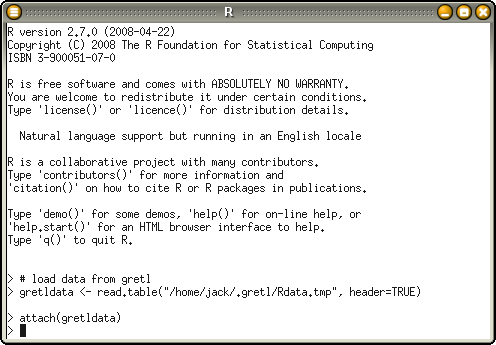
\includegraphics[scale=0.7]{figures/Rwindow-1}
  \caption{\app{R} window}
  \label{fig:Rwind1}
\end{figure}

A few caveats here: the actual look of the \app{R} window may be
somewhat different from what you see in figure \ref{fig:Rwind1}
(especially for Windows users), but this is immaterial. The important
point is that you have a window where you can type commands to
\app{R}. If the above procedure doesn't work and no \app{R} window
opens, it means that \app{gretl} was unable to launch \app{R}: you
should ensure that \app{R} is installed and working on your system and
that \app{gretl} knows where it is. The relevant settings can be found
by selecting the ``Tools, Preferences, General'' menu entry, under the
``Programs'' tab.

Assuming \app{R} was launched successfully, you will notice that two
commands have been executed automatically:
\begin{code}
  gretldata <- read.table("/home/jack/.gretl/Rdata.tmp", header=TRUE)
  attach(gretldata)
\end{code}
These commands make it so that our dataset is already loaded into the
\app{R} workspace as a \emph{data frame} and can be used
immediately. In \app{R} parlance, a data frame is one of the ways
\app{R} uses to store data. The advantage of using a data frame is
that the subsequent \texttt{attach()} command ensures that the
variable names defined in the \app{gretl} workspace are available as
valid identifiers in the \app{R} session.

In order to replicate \app{gretl}'s OLS estimation, select the \app{R}
window and type at the prompt
\begin{code}
  model <- lm(price ~ sqft + bedrms + baths)
  summary(model)
\end{code}

\begin{figure}[htbp]
  \centering
  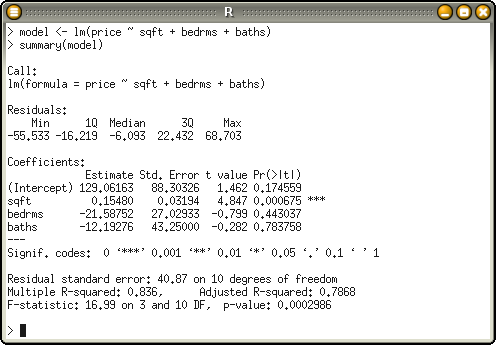
\includegraphics[scale=0.7]{figures/Rwindow-2}
  \caption{OLS regression on house prices via \app{R}}
  \label{fig:Rwind2}
\end{figure}

You should see something similar to Figure
\ref{fig:Rwind2}. Surprise --- the estimates coincide! At this
point, you may just close the \app{R} window or type \verb|q()| at the
\app{R} prompt.

\subsection{Time series data}
\label{sec:R-ols-arma}

Let us now turn to a similar example which uses time series data: we
will compare \app{gretl}'s and \app{R}'s estimates of Box and Jenkins'
immortal ``airline'' model. The data are contained in the \texttt{bjg}
sample dataset. The following \app{gretl} code
\begin{code}
open bjg
arima 0 1 1 ; 0 1 1 ; lg --nc
\end{code}
produces the estimates shown in Table \ref{tab:airline-gretl}.

\begin{table}[htbp]
\caption{Airline model from Box and Jenkins (1976) --- selected
  portion of \app{gretl}'s estimates}
\label{tab:airline-gretl}
\begin{center}

\begin{tabular*}{0.75\textwidth}{@{\extracolsep{\fill}}
l% col 1: varname
  D{.}{.}{-1}% col 2: coeff
    D{.}{.}{-1}% col 3: sderr
      D{.}{.}{-1}% col 4: t-stat
        D{.}{.}{4}}% col 5: p-value (or slope)
Variable &
  \multicolumn{1}{c}{Coefficient} &
    \multicolumn{1}{c}{Std.\ Error} &
      \multicolumn{1}{c}{$t$-statistic} &
        \multicolumn{1}{c}{p-value} \\[1ex]
$\theta_{1}$ &
  -0.401824 &
    0.0896421 &
      -4.4825 &
        0.0000 \\
$\Theta_{1}$ &
  -0.556936 &
    0.0731044 &
      -7.6184 &
        0.0000 \\
\end{tabular*}

\begin{tabular}{lD{.}{.}{-1}}
Variance of innovations & 0.00134810 \\
Log-likelihood & 244.696 \\
Akaike information criterion & -483.39 
\end{tabular}
\end{center}
\end{table}

When we open an \app{R} session as described in the previous
subsection, the data-passing mechanism is slightly different: since
our data were defined in \app{gretl} as a time-series dataset, the
\app{R} object we use for transferring the data is a
\emph{time-series} object, or \emph{ts} for short. The \app{R}
commands that read the data from \app{gretl} are in this case
\begin{code}
# load data from gretl
gretldata <- read.table("/home/jack/.gretl/Rdata.tmp", header=TRUE)
gretldata <- ts(gretldata, start=c(1949, 1), frequency = 12)
\end{code}

This mechanism makes it possible to retain in \app{R} some useful
information, such as the periodicity of the data and the sample
limits, but comes at the price that the names of individual series, as
defined in the \app{gretl} dataset, are not valid identifiers. In
order to extract the variable \texttt{lg}, one needs to use the syntax
\verb|lg <- gretldata[, "lg"]|.

In practice, ARIMA estimation can be carried out by issuing the
following two \app{R} commands:
\begin{code}
lg <- gretldata[, "lg"]
arima(lg, c(0,1,1), seasonal=c(0,1,1))
\end{code}

which yield

\begin{code}
Coefficients:
          ma1     sma1
      -0.4018  -0.5569
s.e.   0.0896   0.0731

sigma^2 estimated as 0.001348:  log likelihood = 244.7,  aic = -483.4
\end{code}

Luckily, the estimates again coincide.

\section{Running an \app{R} script}
\label{sec:R-scripts}

Opening an \app{R} window and keying commands in is a convenient method when
the job is small. In some cases, however, it would be much better to
have \app{R} execute a script prepared in advance. An obvious way to
do this is to use the \texttt{source()} command in
\app{R}. Alternatively, \app{gretl} offers the convenience to edit an
\app{R} script and run it, having the current dataset pre-loaded
automatically. This feature can be accessed via the ``File, Script
Files'' menu entry. By selecting ``User file'', one can load a
pre-existing \app{R} script; if you want to create a new script
instead, select the ``New script, R script'' menu entry.

\begin{figure}[htbp]
  \centering
  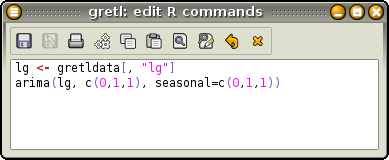
\includegraphics[scale=0.7]{figures/R-edit1}
  \caption{Editing window for \app{R} scripts}
  \label{fig:R-edit1}
\end{figure}
In either case, you will be presented with a window very similar to
the editor window used for ordinary \app{gretl} scripts, as in figure
\ref{fig:R-edit1}. 

There are two main differences: first, you get syntax highlighting for
\app{R}'s syntax instead of \app{gretl}'s. Second, clicking on the
Execute icon (the gears icon), launches an instance of \app{R} in
which your commands are executed.  Before \app{R} is actually run, you
are asked if you want to run \app{R} interactively or not (see Figure
\ref{fig:R-exec-mode}).

\begin{figure}[htbp]
  \centering
  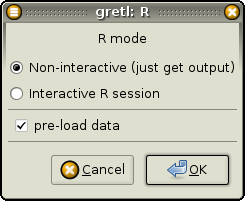
\includegraphics[scale=0.7]{figures/R-exec-mode}
  \caption{Editing window for \app{R} scripts}
  \label{fig:R-exec-mode}
\end{figure}

An interactive run opens an \app{R} instance similar to the one seen
in the previous section: your data will be pre-loaded (if the
``pre-load data'' tick is on, as is by default) and your commands will
be executed. Once this is done, you will find yourself at the \app{R}
prompt, where you can enter more commands.

A non-interactive run, instead, will execute your script, collect the
output at the end of the execution and present it to you in an output
window; \app{R} will be just run in the background. If for example the
script in Figure \ref{fig:R-edit1} is run non-interactively, a window
similar to Figure \ref{fig:R-output1} will appear.

\begin{figure}[htbp]
  \centering
  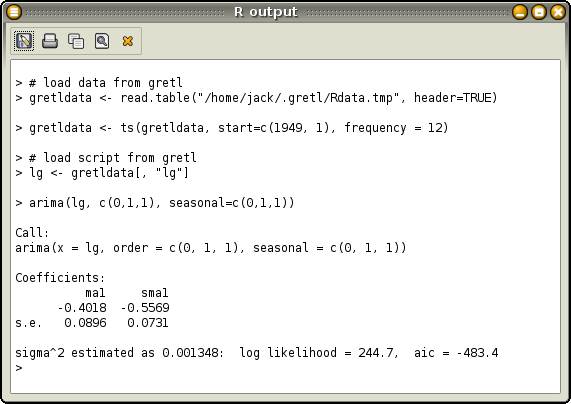
\includegraphics[scale=0.7]{figures/R-output1}
  \caption{Editing window for \app{R} scripts}
  \label{fig:R-output1}
\end{figure}

\section{Taking stuff back and forth}
\label{sec:R-passing-data}

So far, data passing has been limited to passing series from
\app{gretl} to \app{R}. In order to achieve a satisfactory degree of
interoperability, more is needed.

\subsection{Passing matrices from \app{gretl} to \app{R}}

For passing matrices from \app{gretl} to \app{R}, you can use the
\texttt{mwrite} matrix function described in section
\ref{sec:matrix-csv}. For example, the following \app{gretl} code
fragment generates the matrix 
\[ 
A = \left[
  \begin{array}{ccc}
    3 &  7 &  11 \\ 
    4 &  8 &  12 \\ 
    5 &  9 &  13 \\ 
    6 & 10 &  14 
  \end{array}
\right]
\] 
and stores it into the file \texttt{mymatfile.mat}.
\begin{code}
  matrix A = mshape(seq(3,14),4,3)
  err = mwrite(A, "mymatfile.mat")
\end{code}
In order to retrieve this matrix from \app{R}, all you have to do is
\begin{code}
  A <- as.matrix(read.table("mymatfile.mat", skip=1))
\end{code}

It should be noted that although in principle the filename you choose
can be any valid filename, a couple of conventions may prove
useful. First, you may want to use an informative file suffix such as
``\texttt{.mat}'', but this is a matter of taste. More importantly,
the exact location of the file created by \texttt{mwrite} could be an
issue. By default, if no path is specified in the file name,
\app{gretl} stores matrix files in the current work
directory. However, it may be wise for the purpose at hand to use the
directory in which \app{gretl} stores all its temporary files, whose
name is stored in the built-in string \texttt{dotdir} (see section
\ref{sec:named-strings}). The value of this string is automatically
passed to \app{R} as the string variable \texttt{gretl\_dotdir}, so
the above example may be rewritten more cleanly as

\app{Gretl} side:
\begin{code}
  matrix A = mshape(seq(3,14),4,3)
  err = mwrite(A, "@dotdir/mymatfile.mat")
\end{code}
\app{R} side:
\begin{code}
  fname <- paste(gretl_dotdir, "mymatfile.mat", sep="")
  A <- as.matrix(read.table(fname, skip=1))
\end{code}

\subsection{Passing data from \app{R} to \app{gretl}}

For passing data in the opposite direction, \app{gretl} defines a
special function that can be used in the \app{R} environment to
automate, as much as possible, a mechanism which is similar to the one
seen in the previous subsection. An \app{R} object will be written as
a temporary file in \app{gretl}'s \texttt{dotdir} directory, from
where it can be easily retrieved from within \app{gretl}.

The name of this function is \texttt{gretl\_export()}, and it accepts
one argument, the object to be exported. At present, the only objects
that can be exported with this method are matrices, data frames and
time-series objects. The function creates a text file with the same
name as the exported object in \app{gretl}'s temporary directory. Data
frames and time-series objects are stored as CSV files, and can be
retrieved by using the \texttt{append} command. Matrices, instead, are
stored in the special text format that \app{gretl} uses for storing
matrices on text files (see section \ref{sec:matrix-csv}); the file
suffix is in this case \texttt{.mat}, and to read the matrix in
\app{gretl} you must use the \texttt{mread()} function.

As an example, we take the airline data and use them to estimate a
structural time series model \`a la Harvey (1989). The model we will 
use is the \emph{Basic Structural Model} (BSM), in which a time series
is decomposed into three terms:
\[
  y_t = \mu_t + \gamma_t + \varepsilon_t
\]
where $\mu_t$ is a trend component, $\gamma_t$ is a seasonal component
and $\varepsilon_t$ is a noise term. In turn, the following is assumed
to hold:
\begin{eqnarray*}
  \Delta \mu_t & = & \beta_{t-1} + \eta_t \\
  \Delta \beta_t & = & \zeta_t \\
  \Delta_s \gamma_t & = & \Delta \omega_t
\end{eqnarray*}
where $\Delta_s$ is the seasonal differencing operator, $(1-L^s)$, and
$\eta_t$, $\zeta_t$ and $\omega_t$ are mutually uncorrelated white
noise processes. The object of the analysis is to estimate the
variances of the noise components (which may be zero) and to recover
estimates of the latent processes $\mu_t$ (the ``level''), $\beta_t$
(the ``slope'') and $\gamma_t$.

\app{Gretl} does not provide (yet) a command for estimating this class
of models, so we will use \app{R}'s \texttt{StructTS} command and
import the results back into \app{gretl}. Once the \texttt{bjg}
dataset is loaded in gretl, we pass the data to \app{R} and execute
the following script:
\begin{code}
# extract the log series 
y <- gretldata[, "lg"]
# estimate the model
strmod <- StructTS(y)
# save the fitted components
compon <- as.ts(strmod$fitted)
# save the estimated variances
vars <- as.matrix(strmod$coef)

# export into gretl's temp dir
gretl_export(compon)
gretl_export(vars)
\end{code}
%$

Running the above in \app{R} produces
\begin{code}
> # load data from gretl
> gretldata <- read.table("/home/jack/.gretl/Rdata.tmp", header=TRUE)

> gretldata <- ts(gretldata, start=c(1949, 1), frequency = 12)

> # load script from gretl
> #extract the log series 
> y <- gretldata[, "lg"]

> # estimate the model
> strmod <- StructTS(y)

> # save the fitted components
> compon <- as.ts(strmod$fitted)

> # save the estimated variances
> vars <- as.matrix(strmod$coef)

> # export into gretl's temp dir
> gretl_export(compon)

> gretl_export(vars)
\end{code}

At this point, we can pull the results back into \app{gretl} by
executing the following commands, either from the console or by
creating a small script:\footnote{This example will work on Linux
  and presumably on OSX without modifications. On the Windows
  platform, you may have to substitute the ``\texttt{/}'' character
  with ``$\backslash$''.}
\begin{code}
append @dotdir/compon.csv
vars = mread("@dotdir/vars.mat")
\end{code}
The first command reads the estimated time-series components from a
CSV file, which is the format that the passing mechanism employs for
series. The matrix \texttt{vars} is read from the file
\texttt{vars.mat}.

\begin{figure}[htbp]
  \centering
  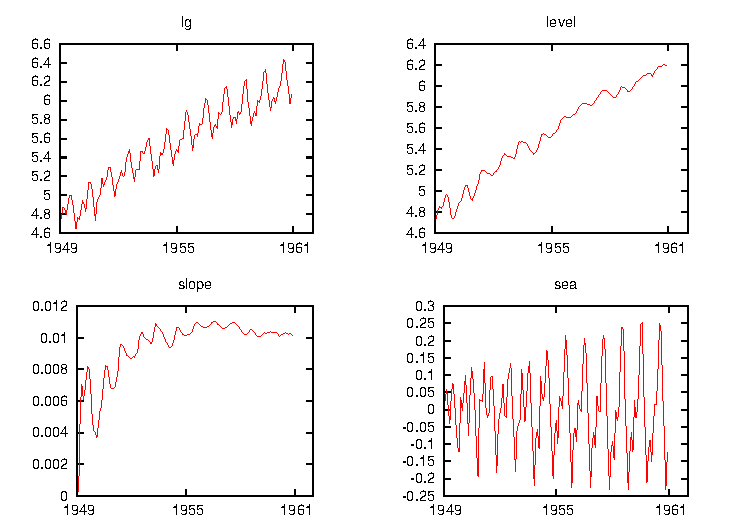
\includegraphics{figures/BSM-output}
  \caption{Estimated components from BSM}
  \label{fig:BSM-output}
\end{figure}

After the above commands have been executed, three new series will
have appeared in the \app{gretl} workspace, which are the estimates of
the three components: by plotting them together with the original
data, you should get a graph similar to Figure
\ref{fig:BSM-output}. The estimates of the variances can be simply
seen by printing the \texttt{vars} matrix, as in

\begin{code}
? print vars
vars (4 x 1)

  0.00077185 
      0.0000 
   0.0013969 
      0.0000 
\end{code}

%%% Local Variables: 
%%% mode: latex
%%% TeX-master: "gretl-guide"
%%% End: 

